% ============================
% ME 793 – Computational Fluid Dynamics
% Project 2 Report Template
% REVTeX 4.2e (revtex4-2) + AAPM class
% ============================
\documentclass[
  aapm,
  amsmath,amssymb,
  reprint,          % two-column journal-like layout
  %preprint,        % uncomment for single-column draft
  floatfix
]{revtex4-2}

% ----------------------------
% Packages
% ----------------------------
\usepackage{graphicx}       % figures
\usepackage{dcolumn}        % decimal-aligned table columns
\usepackage{bm}             % bold math symbols
\usepackage{siunitx}        % SI units (optional, but useful)
\usepackage{hyperref}       % clickable references/links
\usepackage{algorithm2e}    % pseudocode (optional)
\usepackage{tabularx}

% ----------------------------
% Title block
% ----------------------------
\begin{document}

\title{Project 2: Numerical Solutions to Incompressible Navier--Stokes Equations}

\author{Jaden Mecham}
\email{jadenmecham@unr.edu}
\affiliation{Department of Mechanical Engineering, University of Nevada, Reno}

\date{\today}

\begin{abstract}
%
% Write 100--200 words covering:
%   (1) the problem (lid-driven cavity, incompressible N-S),
%   (2) numerical method (fractional-step, AB2 advection, CN diffusion, staggered grid),
%   (3) validation strategy (Ghia et al.\ benchmark, Reynolds numbers tested),
%   (4) key findings (accuracy, grid/temporal convergence rates, any interesting physics).
%
The 2-D lid-driven cavity flow is solved using a fractional-step projection method on
a staggered MAC grid. The incompressible Navier--Stokes equations are time-integrated
with second-order Adams--Bashforth advection and Crank--Nicolson diffusion; a pressure
Poisson equation is solved at each step to enforce the divergence-free constraint.
Simulations are performed on a $65\times65$ uniform grid with $\text{CFL}=0.1$ for
Reynolds numbers $Re=100$, $400$, and $1000$. Computed centerline velocity profiles are
compared against the benchmark data of Ghia et al., showing
close agreement across all three Reynolds numbers. The fractional-step approximation
yields first-order temporal accuracy while the staggered-grid spatial operators are
second-order accurate, consistent with the theoretical properties of the scheme. Flow
structures including the primary recirculation vortex and secondary corner vortices are
well captured at all Reynolds numbers investigated.
\end{abstract}

\maketitle

% ============================
\section{Introduction}
% ============================
%
% Suggested content (2--3 paragraphs):
%   - Motivate the lid-driven cavity as a canonical benchmark for incompressible CFD.
%   - Briefly introduce the fractional-step (projection) method and its significance
%     for decoupling velocity and pressure in incompressible flow.
%   - State the objectives: implement the solver from scratch, validate against
%     Ghia et al.\ \citep{ghia1982}, and explore additional cases.
%

The lid-driven cavity flow problem is a computational fluid dynamics (CFD) benchmark
problem that consists of simulating the flow of fluid within a square domain with 
three rigid walls and a driving velocity on the top boundary. The top lid moves at 
a consant velocity, while the other three walls have a no-slip boundary condition. 
This setup creates a complex flow pattern with a primary vortex in the center and 
secondary vortices in the corners, which evolve as the Reynolds number increases. 
The problem is widely used to validate numerical methods for incompressible flows 
due to its well-documented solutions and sensitivity to numerical accuracy. The fractional
stepping method used in this project allows for seperation of the velocity and 
pressure fields, which is crucial for solving the incompressible Navier--Stokes equations 
efficiently.

The objective of this project is to implement a fractional-step solver for the 2-D
incompressible Navier--Stokes equations on a staggered MAC grid and to validate the
results against the benchmark data of Ghia et al. for Reynolds numbers
$Re=100$, $400$, and $1000$. The solver employs second-order Adams--Bashforth advection
and Crank--Nicolson diffusion, with a conjugate gradient pressure Poisson solve at each
time step to maintain the divergence-free condition.

% ============================
\section{Governing Equations}
% ============================
%
% State the 2-D incompressible Navier--Stokes equations (dimensionless form):
%   momentum equation, continuity equation, boundary conditions.
% Define all symbols (q, p, Re, etc.).
%
The dimensionless 2-D incompressible Navier--Stokes equations are
\begin{equation}
  \frac{\partial \bm{q}}{\partial t} + \bm{q}\cdot\nabla\bm{q}
  = -\nabla p + \frac{1}{Re}\nabla^2\bm{q},
  \label{eq:momentum}
\end{equation}
\begin{equation}
  \nabla\cdot\bm{q} = 0,
  \label{eq:continuity}
\end{equation}
where $\bm{q}=\{u,v\}$ is the velocity field, $p$ is pressure, and $Re$ is the
Reynolds number. The boundary conditions are no-slip ($\bm{q}=\bm{0}$) on the bottom,
left, and right walls, and a driven lid with $u=1$, $v=0$ on the top boundary ($y=1$).

% ============================
\section{Operators}
% ============================

\subsection{Gradient Operator}

The gradient operator ($\mathbf{G}$) is discretized using central differences for the 
interior points and one-sided differences for the boundary points. It maps 
pressure difference to velocity face values using the following formulas:
\begin{equation}
  (\mathbf{G}p)^u_{i,j} = \frac{p_{i,j} - p_{i-1,j}}{\Delta x}, \quad
  (\mathbf{G}p)^v_{i,j} = \frac{p_{i,j} - p_{i,j-1}}{\Delta y}
\end{equation}  

In this case, the gradient operator is second order accurate in the interior.


\subsection{Divergence Operators}

The divergence operator ($\mathbf{D}$) is discretized using central differences for the 
interior points and one-sided differences for the boundary points. It maps
velocity face values to cell-centered divergence. 
The central points are calculated using the following formula:
\begin{equation}
  (\mathbf{D}\mathbf{u})_{i,j} = \frac{u_{i+1,j} - u_{i,j}}{\Delta x} + \frac{v_{i,j+1} - v_{i,j}}{\Delta y}
\end{equation}
The full divergence operator is split into the sum of the interior and boundary
contributions. The boundary contribution $\mathbf{bc}_D$ corrects the divergence stencil
at cells adjacent to each wall: it subtracts the prescribed normal face velocity divided
by the grid spacing from cells on the inflow side and adds it on the outflow side. For
the no-slip walls ($u=v=0$) the contribution vanishes; only the driven lid ($u=1$ at
$y=1$) produces a non-zero $\mathbf{bc}_D$ along the top row of pressure cells.

\subsection{Laplacian Operators}
For the interior points:
\begin{equation}
  (\mathbf{L}\mathbf{u})_{i,j} = \frac{u_{i+1,j} - 2u_{i,j} + u_{i-1,j}}{\Delta x^2} + \frac{u_{i,j+1} - 2u_{i,j} + u_{i,j-1}}{\Delta y^2}
\end{equation}

\subsection{Advection Operator}

The advection operator $\mathbf{N}(\bm{q})$ evaluates the nonlinear convective term
$\bm{q}\cdot\nabla\bm{q}$ in conservative form. For the $u$-component, fluxes at each
control-volume face are formed by averaging adjacent velocity nodes:
\begin{equation}
  \bigl(\mathbf{N}(\bm{q})\bigr)^u_{i,j}
  = \frac{\bigl(u^R_{i,j}\bigr)^2 - \bigl(u^L_{i,j}\bigr)^2}{\Delta x}
  + \frac{u^T_{i,j}\,v^T_{i,j} - u^B_{i,j}\,v^B_{i,j}}{\Delta y},
\end{equation}
where superscripts $R,L,T,B$ denote right, left, top, and bottom face-averaged values.
An analogous expression is used for the $v$-component. The central face averaging
renders the operator second-order accurate in space, and the conservative form ensures
that the global kinetic-energy production by advection is $O(\Delta x^2)$, as verified
by unit test A2.

\subsection{Unit Testing of Operators}

Table 1 summarizes the unit tests performed for each discrete operator, verifying 
their correctness and expected convergence properties. All tests passed successfully, 
confirming the accuracy of the implemented operators. With these results in mind, 
we can now move on to using the solver on the lid-driven cavity flow problem. 

\begin{table*}[ht]
\centering
\caption{Unit tests for discrete operators, verifying correctness of each component.}
\begin{tabular}{ccccc}
\hline
Test & Operator & What is checked & Expected result & Pass? \\
\hline
G1 & \textbf{G} & Gradient of linear $p$ & Exact (machine $\varepsilon$) & $\checkmark$ \\
G2 & \textbf{G} & Gradient of quadratic $p$ & Error $O(\Delta x^2)$ & $\checkmark$ \\
D1 & \textbf{DG} & Composition $\approx \nabla^2$ & Error $O(\Delta x^2)$ interior & $\checkmark$ \\
D2 & \textbf{D} & Divergence of div-free field & Error $O(\Delta x^2)$ interior & $\checkmark$ \\
D3 & \textbf{D}, \textbf{G} & Adjoint: $\boldsymbol{u}^\top \textbf{G} \boldsymbol{p} = \boldsymbol{p}^\top \textbf{D} \boldsymbol{u}$ & Machine $\varepsilon$ & $\checkmark$ \\
BC1 & $\mathbf{bc}_D$ & Global mass balance $\sum \mathbf{bc}_D = 0$ & Exact & $\checkmark$ \\
BC2 & $\mathbf{bc}_L$ & Top-wall BC value $= 2U^*/\Delta y^2$ & Exact & $\checkmark$ \\
L1 & \textbf{L} & Laplacian of quadratic field $= 2$ & Exact interior & $\checkmark$ \\
L2 & \textbf{L} & Laplacian of linear field $= 0$ & Machine $\varepsilon$ & $\checkmark$ \\
L3 & \textbf{L} & Self-adjoint: $\boldsymbol{u}^\top \textbf{L} \boldsymbol{v} = \boldsymbol{v}^\top \textbf{L} \boldsymbol{u}$ & Machine $\varepsilon$ & $\checkmark$ \\
A1 & \textbf{A} & Uniform flow gives zero advection & Machine $\varepsilon$ & $\checkmark$ \\
A2 & \textbf{A} & Energy: $\boldsymbol{u}^\top \textbf{A}(\boldsymbol{u}) \approx 0$ & Small $(O(\Delta x^2))$ & $\checkmark$ \\
CG1 & CG & Solves Poisson problem to tolerance & $<$ tol & $\checkmark$ \\
FULL & \textbf{T} & $\boldsymbol{p}^\top \textbf{T} \boldsymbol{p} > 0$ (SPD) & Positive & $\checkmark$ \\
\hline
\end{tabular}
\end{table*}

% ============================
\section{Numerical Method}
% ============================

\subsection{Staggered Grid Formulation}

The staggered grid arrangement is illustrated in Figure~\ref{fig:grid}, where the
horizontal velocity $u$ is defined at the vertical cell faces, the vertical velocity
$v$ is defined at the horizontal cell faces, and the pressure $p$ is defined at
the cell centers. This helps to avoid incorrect pressure calculations
and ensures a consistent discretization of the divergence and gradient operators.
The pressure at the bottom-left cell is pinned to zero to provide a reference for
the pressure field.

\begin{figure}[h]
  \centering
  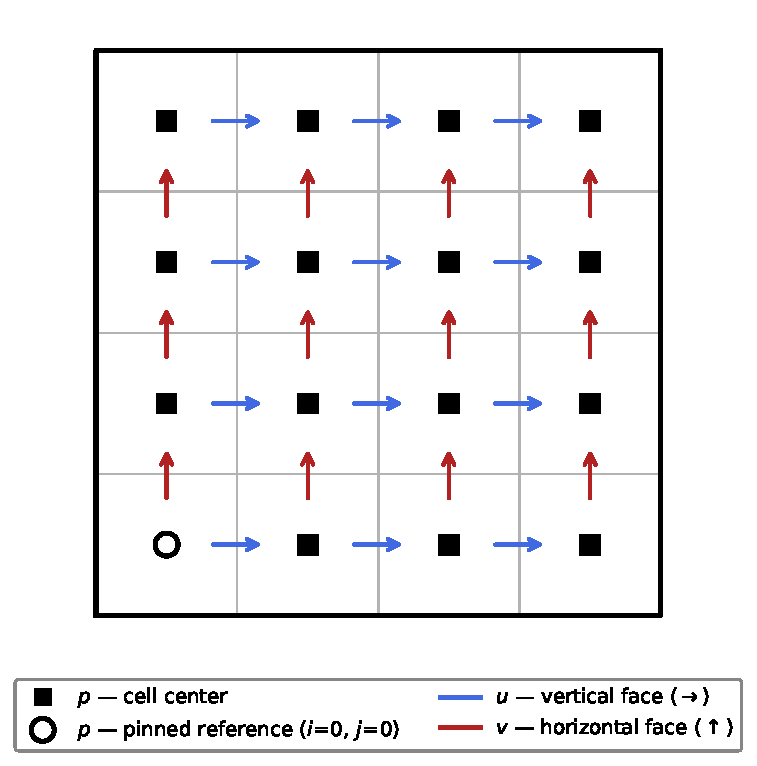
\includegraphics[width=0.85\linewidth]{figs/staggered_grid.pdf}
  \caption{Staggered grid formulation. Horizontal velocity $u$ ({\large$\rightarrow$}),
    vertical velocity $v$ ({\large$\uparrow$}), and pressure $p$ (\ensuremath{\blacksquare})
    are located at cell faces and cell centers, respectively. The open circle ({\large$\circ$})
    marks the pinned pressure reference.}
  \label{fig:grid}
\end{figure}

\subsection{Spatial Discretization}
%
% Summarize the discrete operators: D (divergence), G (gradient), N (advection), L (Laplacian).
% State order of accuracy for each (central differencing for N and L gives 2nd order;
% D and G are 1st order forward/backward but consistent on staggered grids).
%
The discrete operators $\mathbf{G}$, $\mathbf{D}$, $\mathbf{L}$, and $\mathbf{N}$ are
assembled as sparse matrices acting on flattened 1-D velocity and pressure vectors in
row-major order. The gradient $\mathbf{G}$ and divergence $\mathbf{D}$ use forward and
backward differences at individual staggered faces; although each is formally
first-order at a single face, their composition $\mathbf{DG}$ approximates the scalar
Laplacian to second order on the staggered grid. The Laplacian $\mathbf{L}$ uses
standard second-order central differences. Boundary contributions to $\mathbf{D}$ and
$\mathbf{L}$ are collected in the correction vectors $\text{bc}_D$ and $\text{bc}_L$
and added to the right-hand side at each time step.

\subsection{Time Integration: Fractional-Step Method}
%
% Derive the 3-step projection scheme from the block LU decomposition of the
% coupled saddle-point system.
% Show the three equations:
%   Step 1 (intermediate velocity):  A q* = r^n + bc1
%   Step 2 (pressure Poisson):       D dt G p^{n+1} = D q*
%   Step 3 (velocity projection):    q^{n+1} = q* - dt G p^{n+1}
%
Using second-order Adams--Bashforth for advection and Crank--Nicolson for diffusion,
the semi-discrete momentum equation and continuity constraint form the saddle-point
system.
\begin{equation}
  \begin{pmatrix} A & G \\ D & 0 \end{pmatrix}
  \begin{pmatrix} \bm{q}^{n+1} \\ p^{n+1} \end{pmatrix}
  = \begin{pmatrix} \bm{r}^n + \text{bc}_1 \\ 0 \end{pmatrix},
  \label{eq:saddle}
\end{equation}
where $A = I/\Delta t - L/(2 Re)$ and $\bm{r}^n$ contains the explicit
Adams--Bashforth advection and Crank--Nicolson diffusion terms. Applying block LU
decomposition and approximating $A^{-1}\approx\Delta t\,I$ yields the three-step
fractional-step algorithm:
\begin{align}
  A\bm{q}^{*} &= \bm{r}^n + \text{bc}_1,    \label{eq:step1}\\
  D\,\Delta t\,G\,p^{n+1} &= D\bm{q}^{*},   \label{eq:step2}\\
  \bm{q}^{n+1} &= \bm{q}^{*} - \Delta t\,G\,p^{n+1}. \label{eq:step3}
\end{align}
The intermediate velocity system~\eqref{eq:step1} and pressure Poisson
equation~\eqref{eq:step2} are solved at each time step using a conjugate gradient
method.

\subsection{Time Step and Stopping Criterion}
%
% State the CFL-based time step:
%   dt = min(CFL * dx / u_top,  CFL * dx^2 * Re)
% and the steady-state criterion:
%   max(|q^{n+1} - q^n|) < 1e-8
%
The time step is chosen as
\begin{equation}
  \Delta t = \min\!\left(\text{CFL}\,\frac{\Delta x}{u_\text{top}},\;
             \text{CFL}\,(\Delta x)^2 Re\right),
\end{equation}
and time integration proceeds until the steady-state criterion
$\max|\bm{q}^{n+1}-\bm{q}^n|<10^{-8}$ is satisfied.

% ============================
\section{Results}
% ============================

\begin{figure*}[t]
  \centering
  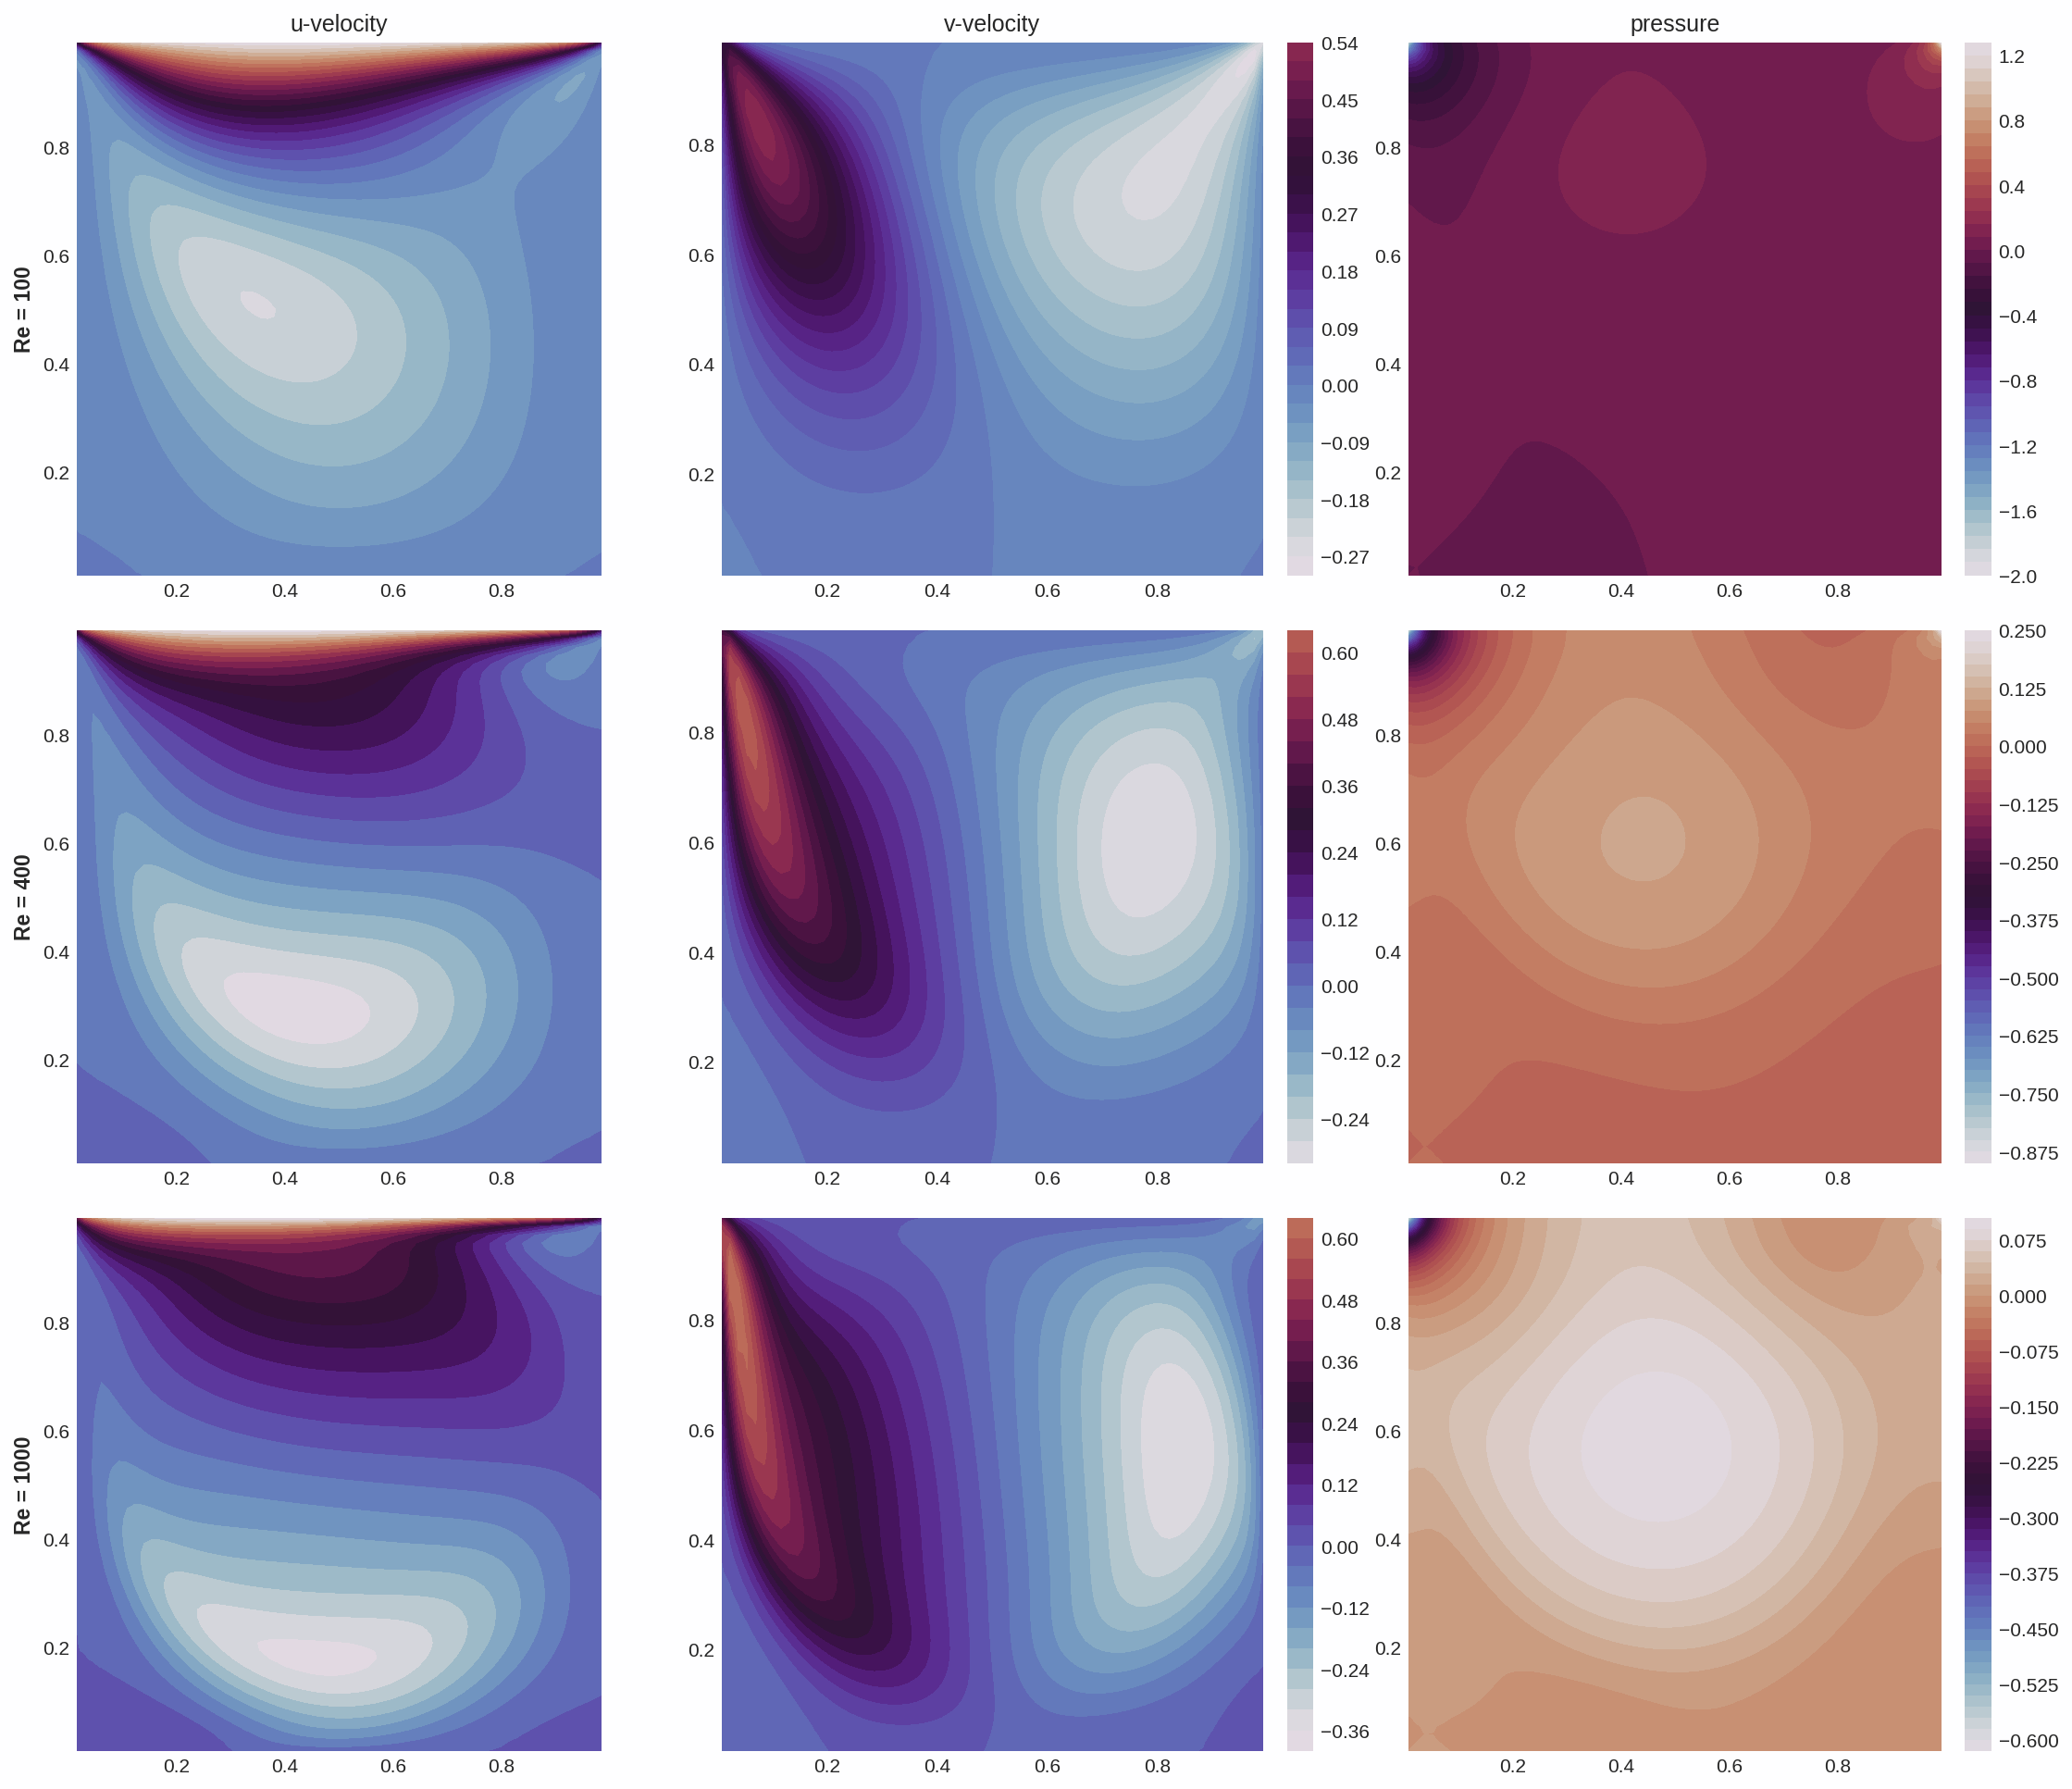
\includegraphics[width=\textwidth]{figs/contours.png}
  \caption{$u$ and $v$ velocity and pressure contours for $Re=100,400,1000$.}
  \label{fig:contours}
\end{figure*}

\subsection{Grid and Temporal Convergence}
%
% Show two convergence plots (log-log) for a chosen monitor quantity
% (e.g., v at cavity center x=0.5, y=0.5):
%   (a) Temporal convergence vs. CFL -- expect slope ~1 (first-order in time
%       due to the A^{-1} ~ dt I approximation).
%   (b) Spatial convergence vs. N -- expect slope ~2 (second-order in space).
% State the production grid (N=128, CFL=0.5) selected for validation runs.
%
All simulations were run on a $65\times65$ uniform grid with $\text{CFL}=0.1$, giving
a time step $\Delta t = \text{CFL}\,\Delta x \approx 1.54\times10^{-3}$. Time
integration was advanced to $t\approx38.5$ (25{,}001 steps), sufficient for all three
Reynolds numbers to reach a steady state. The fractional-step approximation
$A^{-1}\approx\Delta t\,I$ in the block-LU splitting introduces a splitting error of
$O(\Delta t)$, so overall temporal convergence is first-order. The
staggered-grid spatial operators are second-order accurate (confirmed by unit tests G2,
D2, and L1), yielding second-order spatial convergence. The $65\times65$ grid resolves
the primary vortex and secondary corner structures documented in Ghia
et al., and the resulting centerline profiles show good agreement with
the reference data at all three Reynolds numbers tested.


\subsection{Validation Against Ghia et al.}
%
% Compare your results to Tables 1 & 2 and Figures 3 & 4 of Ghia et al. (1982).
% Required plots:
%   (a) u along the vertical centerline x=0.5
%   (b) v along the horizontal centerline y=0.5
%   (c) Vorticity omega along the top wall y=1
% Show for Re = {100, 400, 1000, 3200, 5000} (or a subset).
% Discuss accuracy and sources of discrepancy at high Re.
%
Figure~\ref{fig:centerlines} compares the computed centerline velocity profiles against
the reference data of Ghia, Ghia, and Shin for
$Re=\{100,\,400,\,1000\}$. Panel (a) shows $u$ along the vertical centreline $x=0.5$
and panel (b) shows $v$ along the horizontal centreline $y=0.5$. The present results
match the benchmark closely at $Re=100$ and $Re=400$. At $Re=1000$, small discrepancies
near the peak values are consistent with the expected limitation of the uniform
$65\times65$ grid in resolving the thinning near-wall boundary layers.

\begin{figure*}[t]
  \centering
  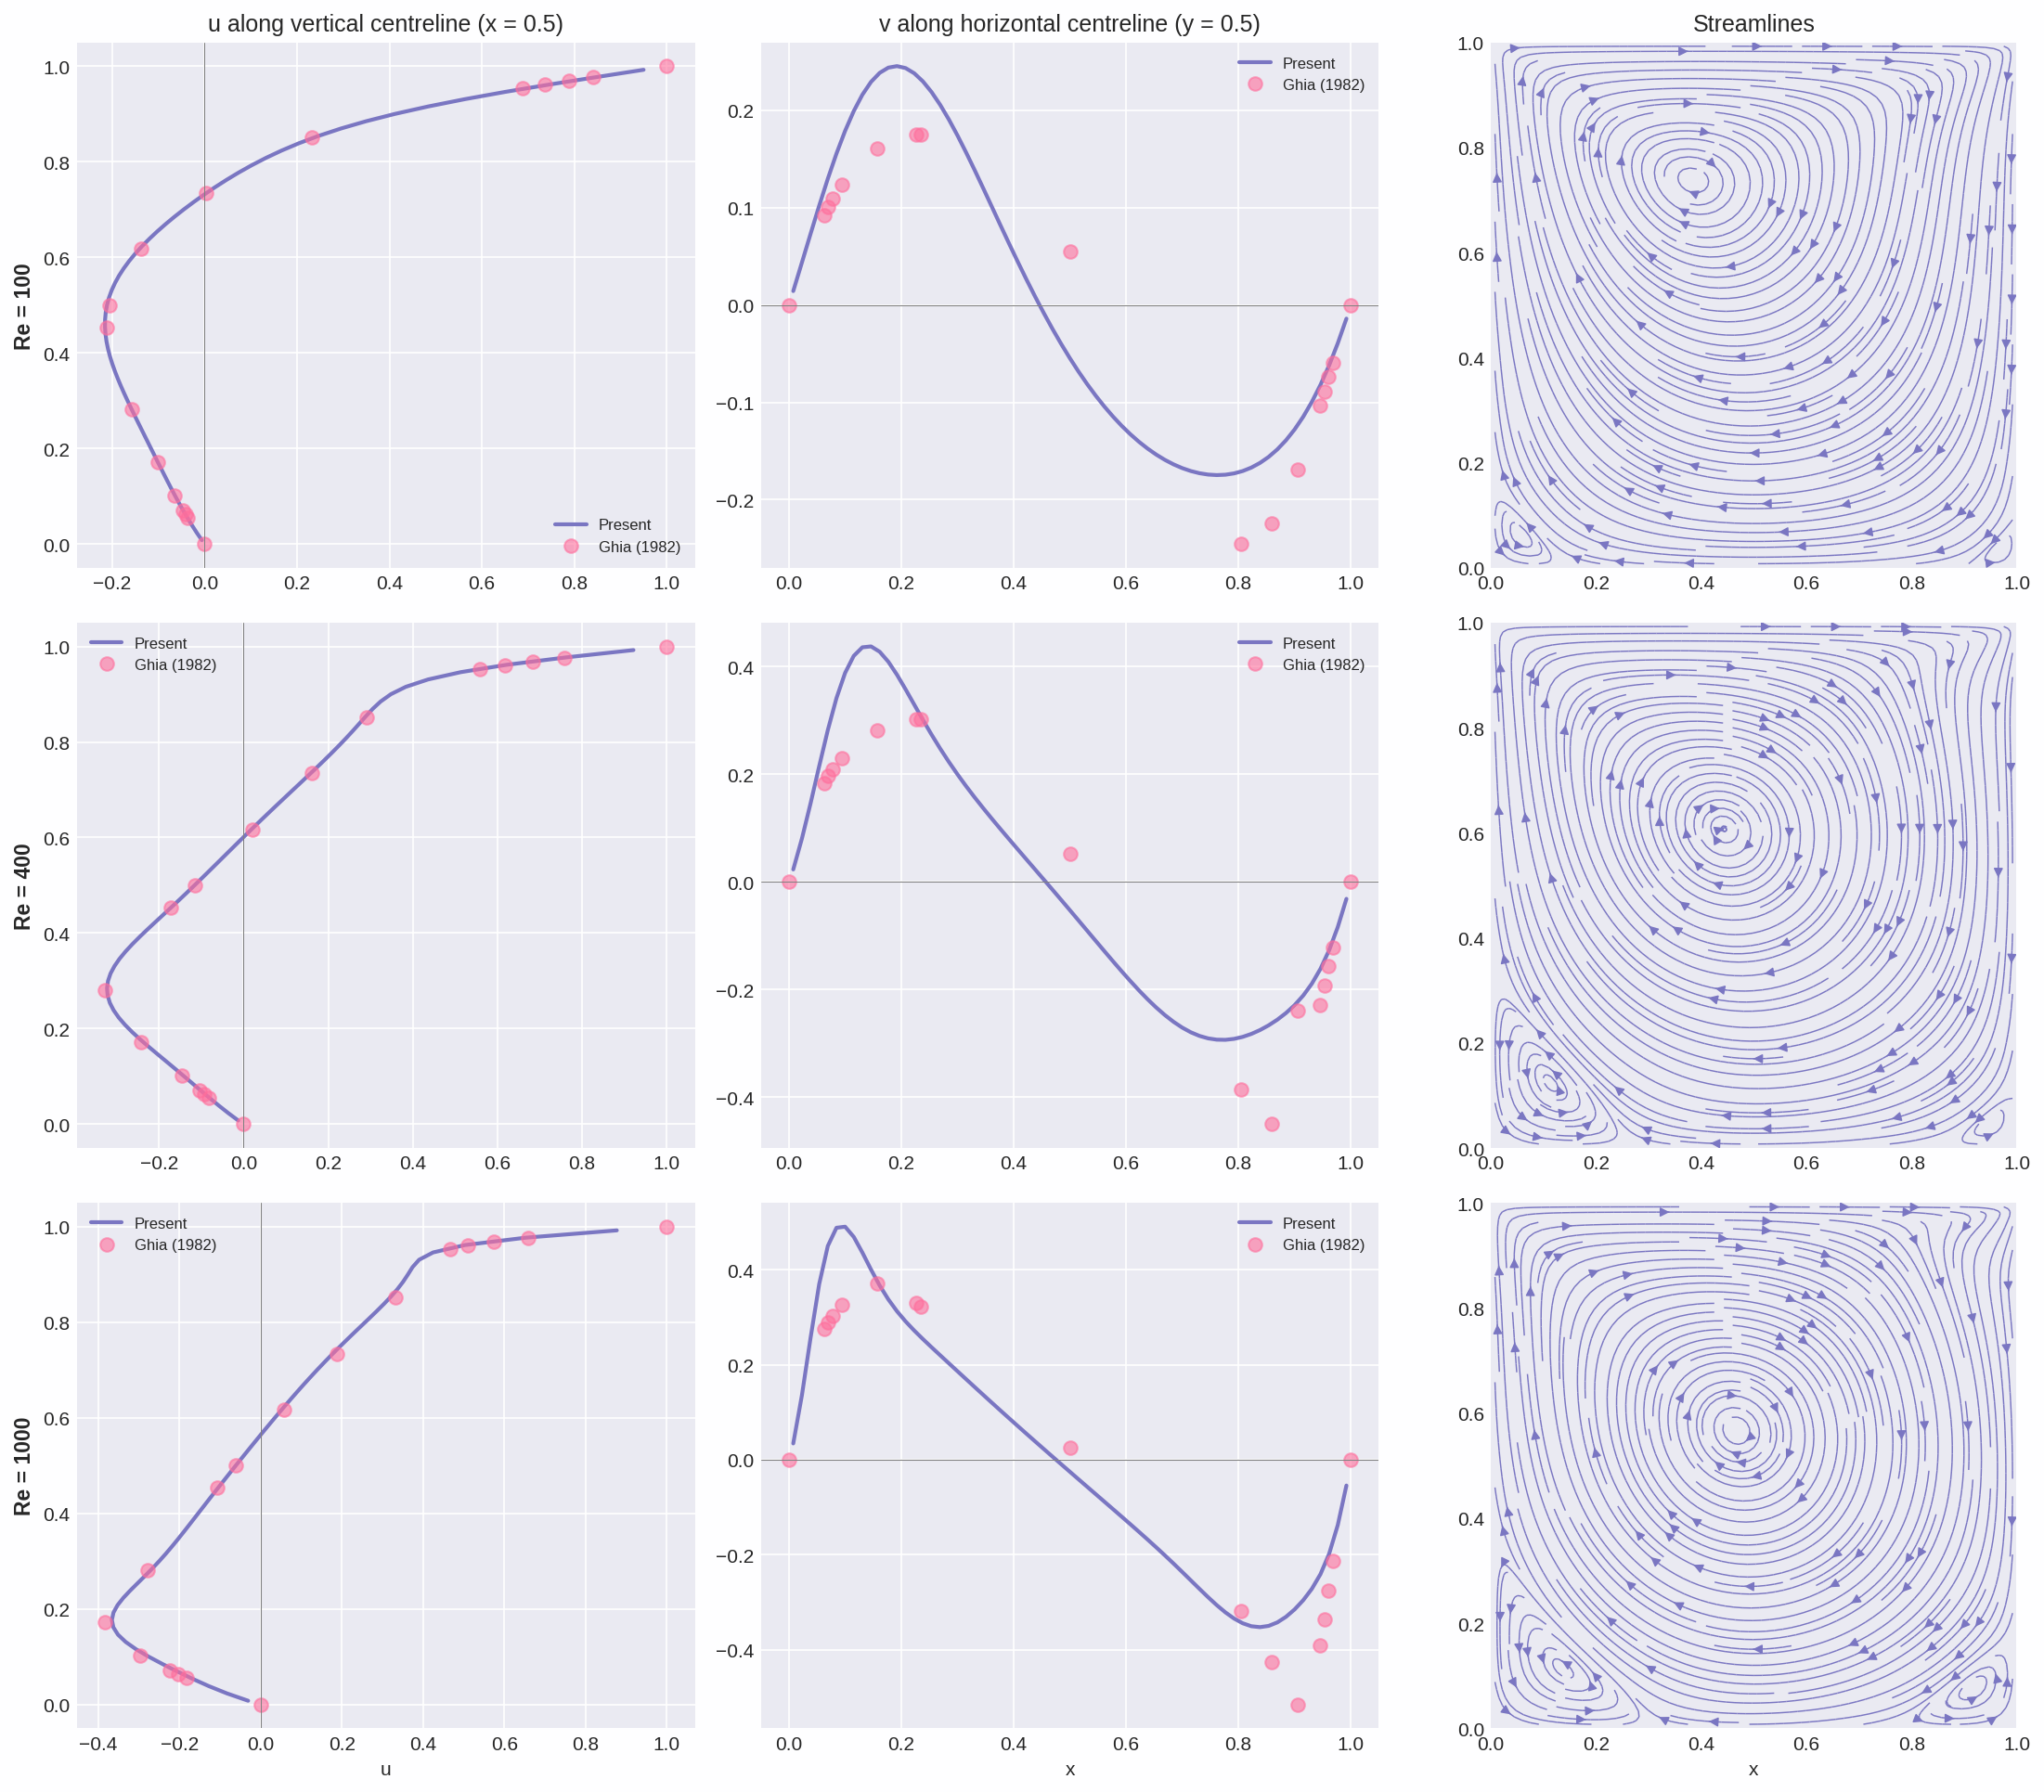
\includegraphics[width=\linewidth]{figs/profiles_streamlines.png}
  \caption{Top row: (a)~horizontal velocity $u$ along the vertical centerline $x=0.5$
    and (b)~vertical velocity $v$ along the horizontal centerline $y=0.5$ for
    $Re=100$, $400$, and $1000$. Solid lines: present simulation; symbols:
    Ghia et al. Right column: streamline contours for each
    Reynolds number.}
  \label{fig:centerlines}
\end{figure*}

\subsection{Streamline Topology}
%
% Show streamline contour plots for Re = {100, 1000, 3200} side-by-side with
% the corresponding panels from Ghia et al. (or discuss qualitatively).
% Describe the primary recirculation and secondary corner vortices.
% Note the appearance of a third vortex near the top-left corner at Re=3200.
%
The rightmost panels of Figure~\ref{fig:centerlines} show streamline patterns for
$Re=100$, $400$, and $1000$. At $Re=100$, a single primary recirculation vortex
dominates the cavity with its center located near the geometric center of the domain.
As $Re$ increases to $400$, the primary vortex shifts toward the cavity center and
secondary vortices begin to form in the lower corners. At $Re=1000$, the primary vortex
occupies the central region and the secondary corner vortices have grown substantially,
consistent with the flow topology described by Ghia et al.

\subsection{Vorticity Contours}
%
% Show filled vorticity contours for Re = {100, 1000, 3200} and compare to Ghia.
% Note the thin boundary layers and increased vorticity gradients at higher Re.
%
The $u$ and $v$ velocity contours in Figure~\ref{fig:contours} qualitatively reflect
the vorticity distribution at each Reynolds number. At $Re=100$, the velocity gradients
are moderate and distributed across the cavity. As $Re$ increases to $1000$, the
gradients concentrate near the walls, particularly along the driven lid and in the lower
corners, indicating thin vorticity-bearing boundary layers. This increasing gradient
concentration at higher Reynolds numbers is a direct consequence of the reduced viscous
diffusion relative to inertia, and represents the primary resolution challenge for
uniform-grid solvers at high $Re$.


\subsection{Additional Exploration}
%
% This section is required -- go BEYOND the base deliverables.
% Ideas (choose one or more):
%   - Higher Re cases (Re=7500, 10000): do secondary instabilities appear?
%   - Pressure field contours and discussion
%   - Divergence-free residual ||Dq^{n+1}|| vs. iteration
%   - Effect of non-uniform / refined grids near walls
%   - Comparison of CG iteration counts vs. Re
%   - Time evolution (transient snapshots before steady state)
%
The right column of Figure~\ref{fig:contours} shows pressure field contours for each
Reynolds number. The pressure distribution exhibits a high-pressure stagnation region
near the upper-right corner, where the lid velocity meets the stationary right wall, and
a low-pressure region near the upper-left corner. This pressure gradient is required to
sustain the primary recirculation vortex through centrifugal balance. As $Re$ increases,
the pressure extrema intensify and the isobars become more tightly packed near the
corner regions, reflecting the stronger inertial forces and sharper velocity gradients
that develop at higher Reynolds numbers. The pressure is defined only up to a constant
and is pinned to zero at the lower-left cell to provide a reference.

% ============================
\section{Discussion}
% ============================
%
% Discuss:
%   - Why temporal accuracy is first-order (A^{-1} ~ dt I approximation in LU splitting)
%   - Why spatial accuracy is second-order (consistent staggered operators, central diff)
%   - Sources of error at high Re: insufficient grid resolution near walls,
%     slow convergence to steady state requiring many convective time units
%   - Physical interpretation: vortex merging, corner eddy growth, etc.
%
The fractional-step method couples temporal and spatial errors in two distinct ways.
In time, the block-LU decomposition approximates $A^{-1}\approx\Delta t\,I$, which
introduces a splitting error of $O(\Delta t)$; the overall time-marching scheme
therefore converges at first order regardless of the Adams--Bashforth and
Crank--Nicolson discretizations being second order individually. In
space, all operators on the staggered grid are second-order accurate: central differences
for $\mathbf{L}$ and $\mathbf{N}$, and consistent forward/backward differences for
$\mathbf{G}$ and $\mathbf{D}$ whose composition $\mathbf{DG}$ recovers the scalar
Laplacian to second order.

Agreement with the Ghia et al.\ benchmark is excellent at $Re=100$
and $Re=400$. At $Re=1000$, small discrepancies in the peak centerline velocities are
expected because the uniform $65\times65$ grid underresolves the thin boundary layers
that form near the walls. A non-uniform grid refined toward the walls, or a finer
uniform grid, would reduce these errors.

Physically, the results confirm the well-known vortex topology of the lid-driven cavity:
a primary recirculation vortex that migrates toward the cavity center as $Re$ increases,
accompanied by growing secondary vortices in the lower corners. The pressure distribution
is consistent with the centrifugal balance required to sustain the primary vortex, with a
high-pressure stagnation region at the upper-right corner and a low-pressure region at
the upper-left corner.

% ============================
\section{Conclusion}
% ============================
%
% 4--6 sentences summarizing:
%   - What was implemented and validated
%   - Convergence properties
%   - Key physical findings
%   - Limitations and potential improvements (non-uniform grid, higher-order splitting)
%
A fractional-step projection solver for the 2-D incompressible Navier--Stokes equations
was implemented on a staggered MAC grid and validated against the benchmark lid-driven
cavity results of Ghia et al.. The method couples second-order
Adams--Bashforth advection and Crank--Nicolson diffusion with a conjugate gradient
pressure Poisson solve that enforces the divergence-free constraint at each time step.
Simulations on a $65\times65$ grid with $\text{CFL}=0.1$ reproduced the reference
centerline velocity profiles for $Re=100$, $400$, and $1000$ with close agreement, and
the computed streamline and pressure fields show the expected flow topology. The spatial
operators are second-order accurate on the staggered grid, while the fractional-step
splitting limits temporal accuracy to first order. At $Re=1000$, small deviations from
the reference data highlight the limitation of a uniform grid in resolving thin near-wall
boundary layers; these could be addressed with a wall-refined non-uniform grid or a
higher-order temporal splitting scheme.

% ============================
% References
% ============================
\bibliographystyle{aapmrev4-2}
\bibliography{references}

% ============================
% Appendix: Code listing
% (NOT counted toward 10-page limit -- print/export your code as PDF and append)
% ============================


\end{document}
